\chapter{Arithmetic}

A library of efficient commonly used arithmetic functions is needed for efficient circuit generation.
Further it is useful to have in-place functions whenever possible. 

\section{Addition}
  An addition circuit is a circuit which takes two $n$ bit integers $a = a_1a_2\dotsc a_n$ and $b = b_1b_2\dotsc b_n$ and returns the sum $a+b$. 
  \subsection{Classic Ripple} 
    The classic ripple addition method simply adds the bits in each column starting from the least significant bit.
    The output for that bit is the result modulo 2 and a carry is set to be added to the next column if the result is $>1$.

    To preform this algorithm we will need a circuit that takes three bits then calculates a carry and a sum.
    These can then be applied iteratively taking the two bits from the column of the numbers that are to be added as well as the previous carry.
    
    This can be done with a full adder circuit.
    A full adder is a circuit which takes input bits $a$, $b$, and $c$ then returns the sum ($a \oplus b \oplus c$) as well as the carry ($ab\oplus ac \oplus bc$).
    In figure~\ref{fig:classicalFA} an irreversible implementation can be seen.
    \begin{figure}[ht]
        \capstart
        \centering 
        \begin{circuitikz} \draw
            (3,0) node[xor port] (abxor) {}
            (6,-0.5) node[xor port] (abcxor) {}
            (6,-2) node[and port] (caband) {}
            (6,-3.5) node[and port] (aband) {}
            (8,-2.75) node[or port] (carryor) {}
            (0,0) node[anchor=east] (a) {$a$}
                to[short, o-*] (0.5,0)   
                -| (abxor.in 1)
                (0.5,0)  |- (aband.in 1)
            (0,-0.5) node[anchor=east] (b) {$b$}
                to[short, o-*] (1,-0.5)    
                (1,-0.5) -| (abxor.in 2)
                (1,-0.5) |- (aband.in 2)
            (0,-1) node[anchor=east] (c) {$c$}
                to[short, o-*] (1.5,-1)   
                (1.5,-1) |- (abcxor.in 2)
                (1.5,-1) |- (caband.in 2)
            (abxor.out) to[short,-*] (3.5,0)
                (3.5,0) -| (abcxor.in 1)
                (3.5,0) |- (caband.in 1)
            (aband) -| (carryor.in 2)
            (caband) -| (carryor.in 1)
            (abcxor.out) node[anchor=west] {Sum}
            (carryor.out) node[anchor=west] {Carry}
            ;
        \end{circuitikz}
        \caption{Irreversible full adder}
        \label{fig:classicalFA}
    \end{figure}
    In the reversible case a circuit (see figure~\ref{fig:reversibleFA}) can be constructed that preforms the mapping: 
    \[
        (a,b,c,0) \mapsto (a,b,a\oplus b\oplus c,ab\oplus ac \oplus bc)
    \]  
    \begin{figure}[ht]
        \capstart
        \centering 
        \[
          \Qcircuit @C=1em @R=.7em {
              \lstick{a} & \ctrl{3} & \ctrl{2} & \qw      & \qw      & \rstick{a}\qw\\
              \lstick{b} & \qw      & \qw      & \ctrl{2} & \ctrl{1} & \rstick{b}\qw\\
              \lstick{c} & \ctrl{1} & \targ    & \ctrl{1} & \targ    & \rstick{a  \oplus b  \oplus c}\qw\\
              \lstick{0} & \targ    & \qw      & \targ    & \qw      & \rstick{ab \oplus ac \oplus bc}\qw
          }
        \]
        \caption{Reversible full adder}
        \label{fig:reversibleFA}
    \end{figure}
    These can then be chained together as they are in the irreversible case.  
    The result will be a circuit which takes inputs $(a,b)$ and produces outputs $(a,b,a+b)$.

\subsection{In-Place Ripple}
    It is sometimes the case that one of the input values is unneeded after the operation.
    In that case it would save space to overwrite the value.
    To do this we could try to construct adder which maps inputs $(a,b)\mapsto(a,a+b)$.

    Such an adder is described in Cuccaro et al.\cite{CDKM:2004} (Note that not all the optimizations described in the original paper are desirable with our gate set as we wish to maximize shared controls). 
    It is very similar to the classic ripple.
    The main improvement is the realization that information about the carry could be stored in one of the input bits of each column.
    This allows it to overwrite one of it's inputs with the resulting sum.
    The circuit uses two main operations: MAJ, and UMA (See figure~\ref{fig:majuma}).
    The MAJ operation takes an input carry $c$ and two input bits $a$ and $b$.
    It computes the carry onto $a$ and partially computes the sum on $b$, it leaves $c$ in an unclean state to be fixed later. 
    This circuit can be repeated and rippled through all of the columns.
    After that is done the UMA operation can be preformed.
    This operation cleans up $a$ and $c$ then finishes computing the sum on $b$. 

    \begin{figure}[ht]
        \capstart
        \centering 
        \begin{subfigure}{.45\textwidth}
            \centering 
            \[
              \Qcircuit @C=1em @R=.7em {
                 \lstick{c} & \qw          & \targ      & \ctrl{2} & \rstick{c \oplus a}\qw\\
                 \lstick{b} & \targ        & \qw        & \ctrl{1} & \rstick{b \oplus a}\qw\\
                 \lstick{a} & \ctrl{-1}    & \ctrl{-2}  & \targ    & \rstick{ab \oplus ac \oplus bc}\qw 
              }
            \]
            \caption{MAJ}
        \end{subfigure}
        \begin{subfigure}{.45\textwidth}
            \centering 
            \[
              \Qcircuit @C=1em @R=.7em {
                  & \ctrl{2} & \targ      & \ctrl{1} & \qw\\
                  & \ctrl{1} & \qw        & \targ    & \qw\\
                  & \targ    & \ctrl{-2}  & \qw      & \qw 
              }
            \]
            \caption{UMA}
        \end{subfigure}
        \caption{}
        \label{fig:majuma}
    \end{figure}

\section{Controlled Ripple}
    This is a simple Controlled addition circuit with a gate count and depth $\Theta(n)$.
    \begin{figure}[ht]
      \capstart
      \centering
      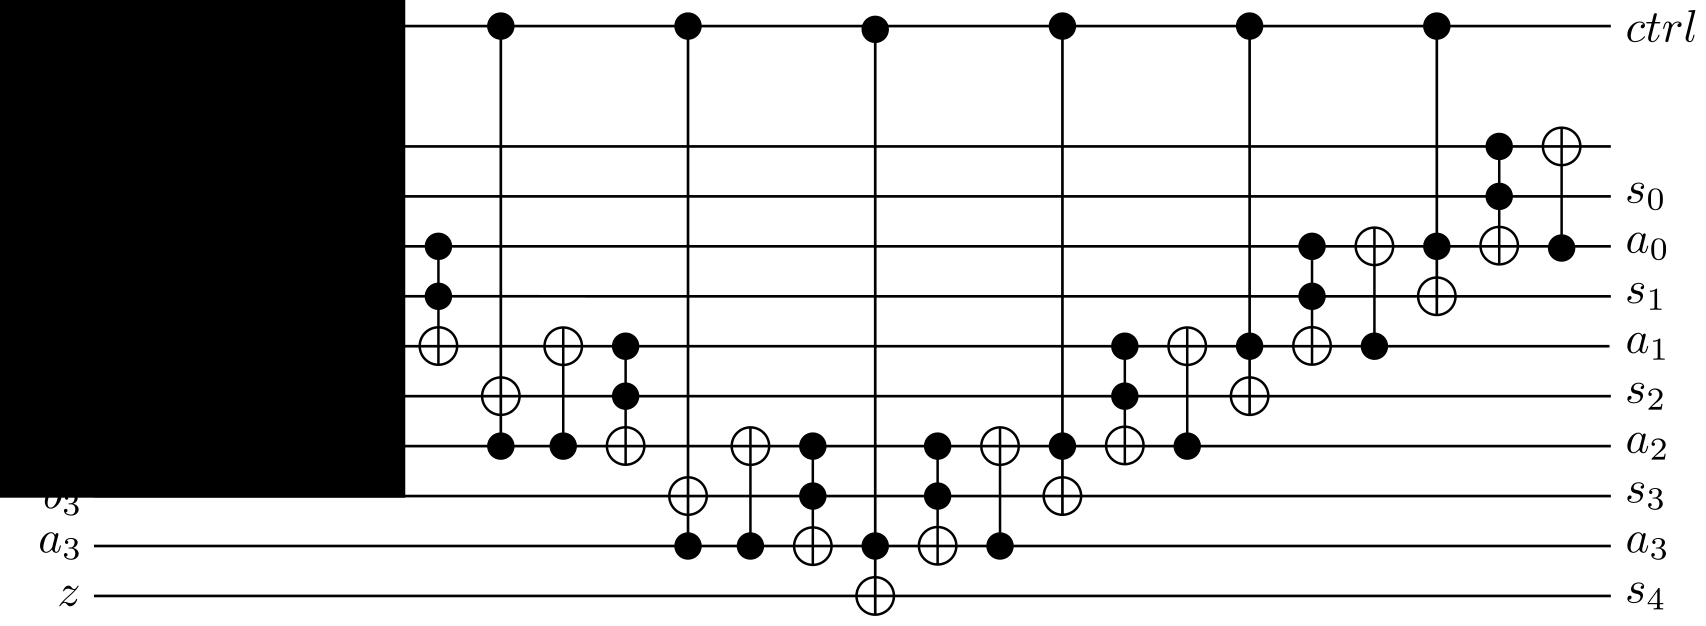
\includegraphics[width=\textwidth]{images/4BitRippleAdderCtrl} 
      \caption{Controlled In-Place Ripple Adder}
      \label{fig:ctrlRipple}
    \end{figure}
    \subsection{Analysis}
      This modification can be accomplished by changing $2n+1$ CNOT gates into Toffoli gates as shown in \cref{fig:ctrlRipple}.
 		  This gives a controlled addition circuit of size $n$ ($A^{ctrl}_n$) a total gate count:
      \begin{align} \label{eq:cadd}
        A^{ctrl}_n = 4n+1
      \end{align}


\section{Multiplication}
  \subsection{Controlled Addition Multiplier}
    A very simple implementation of multiplication as a controlled addition circuit (see figure \ref{fig:ctrlRipple}).  
    Given two numbers as bit strings $a$ and $b$ their product can be found by repeatedly shifting forward by one and adding $b$ to the result controlled on the next bit in $a$.
    See figure \ref{fig:multAdd} for a four bit example.

    This is an out of place multiplier that uses only 1 additional ancilla for the adder circuits.
    \begin{figure}[ht]
      \capstart
      \centering
      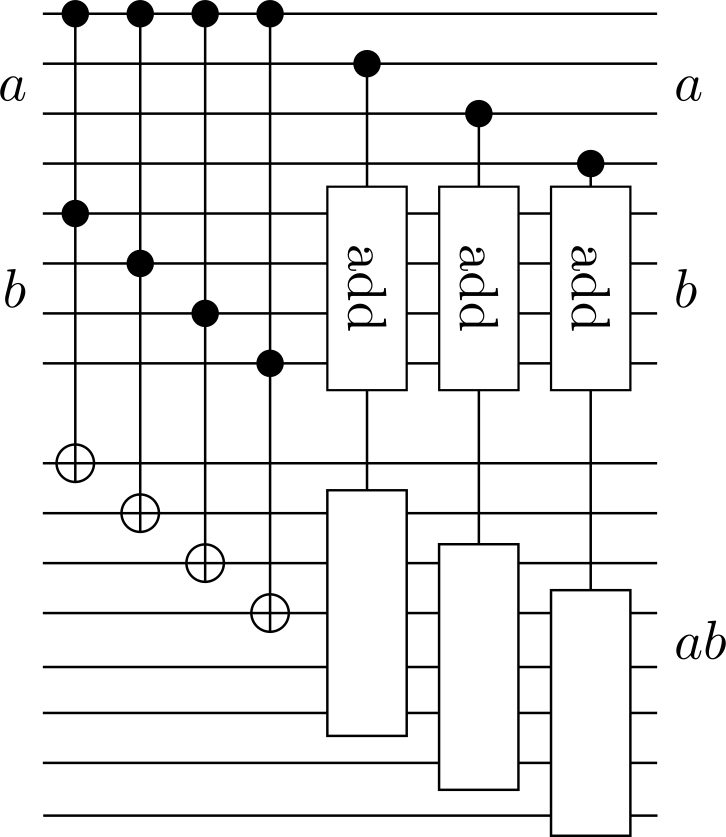
\includegraphics[scale=0.25]{images/multCtrlAdd} 
      \caption{Controlled Addition Multiplier}
      \label{fig:multAdd}
    \end{figure}
    \subsubsection{Analysis}
      This circuit takes $n$ Toffoli gates to copy down the initial value.  
      It then uses $n-1$ controlled in place addition circuits to produce the final value.
        
      So if we define $A^{ctrl}_n$ to be the Toffoli count for a controlled adder of size $n$ we get $M_n = n + (n-1)A^{ctrl}_n$
      Where $M_n$ is the gate count for a controlled addition based multiplication circuit of size $n$.
      From \eqref{eq:cadd} we know the controlled addition circuit uses $4n+1$ Toffoli gates this gives a full count:
      \begin{align} \label{eq:caddtoff}
        M_n = 4n^2 -2n -1
      \end{align} 
 
\subsection{Quantum Karatsuba}
    Let $n\geq 1$ and let $x$ and $y$ be $n$-bit integers. 
    The well-known Karatsuba\cite{KO:1963} algorithm is based on the observation that by writing $x=x_1 2^{\lceil n/2\rceil}+x_0$ and $y=y_1 2^{\lceil n/2\rceil }+y_0$ the product $xy$ can be evaluated as $xy=2^n A + 2^{\rceil n/2 \rceil} B + C$, where 
    \begin{align*}
      A &= x_1 y_1, \\
      B &= (x_0+x_1)(y_0+y_1) - x_0 y_0 - x_1 y_1,\\
      C &= x_0 y_0. \\
    \end{align*}
    \begin{figure}[ht]
      \capstart
      \centering
      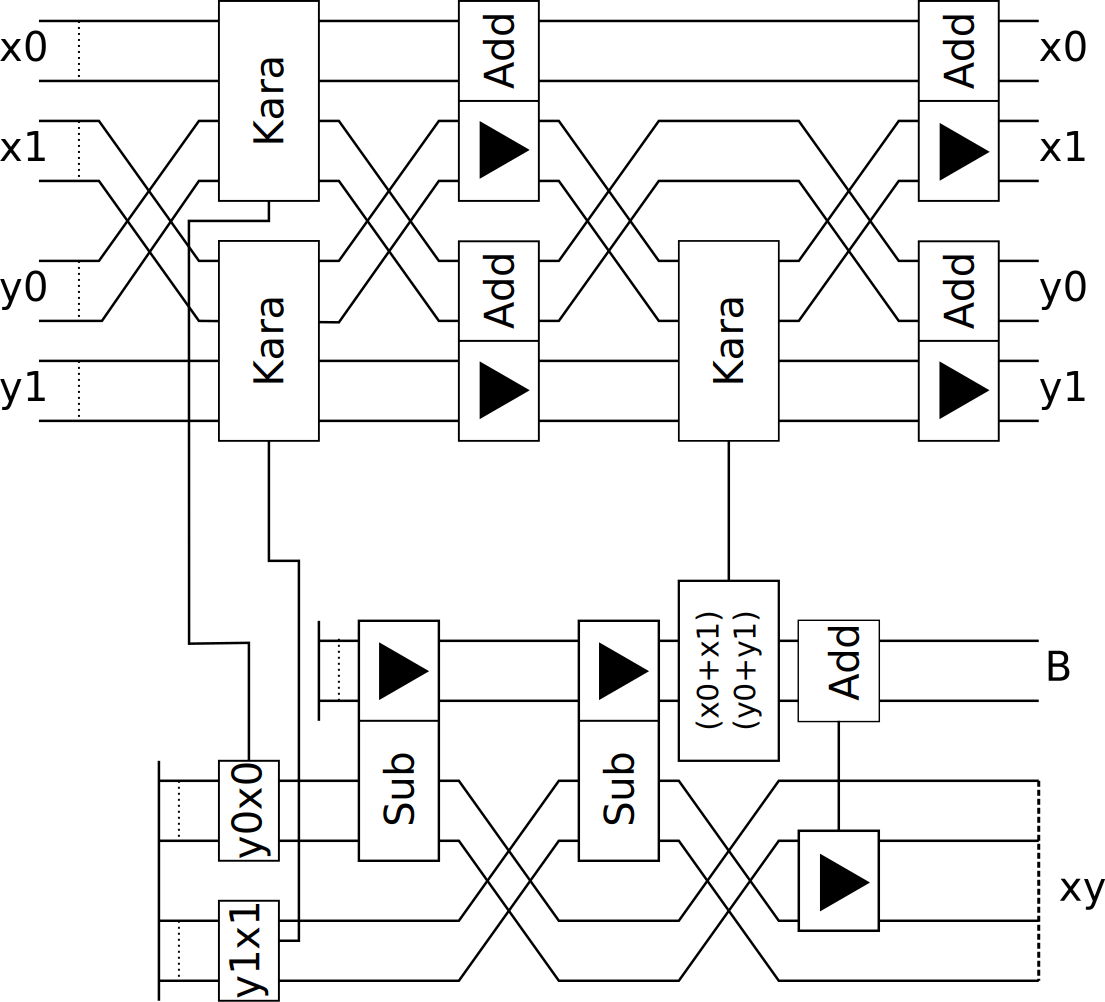
\includegraphics[width=2\textwidth/3]{images/karatsuba2} 
      \caption{Karatsuba Multiplication Circuit.
               Note: In the above circuit notation the black part of the box designates the modified bits in the adder.}
      \label{fig:kara2}
     \end{figure}
    \subsubsection{Analysis}
      Note that the cost for the computation of $A$, $B$, and $C$ are $3$ multiplications and four additions . 
      Note further that the additions to compose the final result do not have to be carried out as the bit representation of $xy$ is the concatenation of the bit representations of $A$, $B$, and $C$. 
      For $m\geq 1$, let $M^{g}_m$ denote the Toffoli cost of a circuit that multiplies $m$-bit inputs $x$ and $y$ using ancillas, i.e., a circuit that maps $(x, y, 0, 0) \mapsto (x, y, g(x,y), xy)$, where $xy$ is a $2m$-bit output, and $g(x,y)$ is an garbage output on $k\geq 1$ bits. 
      Furthermore, denote by $A_m$ the cost for an (in-place) adder of two $m$-bit numbers. 
      It is known that $A_m$ can be bounded by at most $2m$ Toffoli gates. Let $K_n$ denote the number of Toffoli gates that arise in the quantum Karatsuba algorithm (See fig \cref{fig:kara2}).
      The outputs of one step of the recursion are $x_0$,$x_1$, $y_0$, $y_1$, $x_0y_0$, $x_1 y_1$, and $xy$. 
      It is easy to see that allowing garbage, $K_n^g$ can be implemented using $3$ multipliers of half the bit size, $4$ in-place adders of size $n$ and $4$ in place adders of size $n/2$ (note the subtracters are just reversed adders). 
      The base case is a multiplier for two one-bit numbers which can be done with one Toffoli gate, i.e., $K_1^{g}=1$. 
      We obtain the following recursion: 
      \begin{align}
        K_n^{g} = 3 K_{n/2}^{g} + 4 \left(A_{n} + A_{n/2}\right); \quad K_1^{g}=1.
      \end{align}
      For the overall clean implementation of the Karatsuba algorithm we first run this circuit forward, copy out the final result using $n$ CNOTs, and then run the whole circuit backward. 
      This leads to an overall cost of $K_n = 2 K_n^{g}$ and $n$ CNOTs. 
      For the moment we focus on the Toffoli cost only. 
      By expansion we obtain that:
      \begin{align}
        K_n^{g} &= 3^{\log_2(n)} K_1^{g} + 4\left( A_{n}+ A_{n/2} \right) + 12\left( A_{n/2}+ A_{n/4} \right)\notag\\ 
                & + \ldots + 4 \cdot 3^{\log_2(n)-1} \left(A_2 + A_1\right)
      \end{align}
      Using that the Toffoli cost of $A_{n/2^i}$ is $2(n/2^i)$, we obtain for the overall Toffoli cost the following bound: 
      \begin{align}
        K_n &= 2\left(3^{\log_2 n } + 4 \sum_{i=0}^{\log_2 n - 1} 3^i 2(3n/2^i)\right)\notag\\
            &= 2n^{\log_2 3} + 48n \left(\frac{1- (3/2)^{\log_2 n}}{1-3/2}\right) \notag\\
            &= 2n^{\log_2 3} + 96n \left((3/2)^{\log_2{n}} -1\right) \leq 98 n^{\log_2{3}}
      \end{align}
      This bound can be improved by replacing the recursive call to Karatsuba with an instance of some naive multiplication once a certain cutoff has been reached. 
      Looking at \cref{fig:cutoff} we see a comparison of various cutoff values (the naive method is also plotted for reference). 

      Another way to improve this algorithm is to attempt to choose more intelligent splits rather then always splitting the inputs in half at each level.
      This is important because the bit length of the numbers we are adding together may not be a power of two so dividing the input in two at each level might not be optimal.
      In figure \ref{fig:cutoff} the line plotted as \verb+AKara10+ shows the result of using the optimal splits at each level.
      These were found by a simple dynamic program which evaluated the total gate size for every possible split at every level and chose the optimal ones.
		
      As using these methods we find an optimal cutoff value of 11 (see figure \ref{fig:cutoffs}).
      \begin{figure}[ht]
        \centering
        \begin{subfigure}[b]{0.45\textwidth}
        \capstart
        \begin{tikzpicture}[scale=0.5]
          \begin{axis}[
            xlabel={Cutoff},
            ylabel={Average Circuit Size (interval 50 - 500)},
          ]
            \addplot[blue] table {data/cutoffs.dat};
          \end{axis}
        \end{tikzpicture}
        \caption{Average circuit size over the interval 50-500 for various cutoff values}
        \label{fig:cutoffs}
      \end{subfigure}
      \hfill
      \begin{subfigure}[b]{0.45\textwidth}
        \capstart
        \begin{tikzpicture}[scale=0.5]
          \begin{axis}[
            xlabel={Input Size},
            ylabel={Toffoli Gates},
          ]
            \addplot[green] table {data/akara9.dat};
            \addplot[purple] table {data/akara15.dat};
            \addplot[blue] table {data/akara25.dat};
          \end{axis}
        \end{tikzpicture}
        \caption{Comparison of various cutoffs for the adaptive cutoff version.}
        \label{fig:aKara}
      \end{subfigure}
      \caption{}
      \end{figure}

   \subsubsection{Time-Space Tradeoffs}
     We see in figures \ref{fig:cutoff} and \ref{fig:size} that there are trade-offs available between circuits size and gate count available by changing the cutoff value.
  \subsection{Comparison of Multipliers}
    \subsubsection{Gate Count}
      The Karatsuba multiplier has the lowest asymptotic gate count of the circuits discussed.
     \begin{figure}[ht]
        \capstart
        \centering
        \begin{tikzpicture}
          \begin{axis}[
            xlabel={Input Size},
            ylabel={Toffoli Gates},
            legend pos=north west,
          ]
            \addplot[green] table {data/skara5.dat};
            \addlegendentry{sKara 5}
            \addplot[blue] table {data/skara9.dat};
            \addlegendentry{sKara 9}
            \addplot[red] table {data/skara20.dat};
            \addlegendentry{sKara 20}
            \addplot[purple] table {data/skara50.dat};
            \addlegendentry{sKara 50}
            \addplot[brown] table {data/akara9.dat};
            \addlegendentry{aKara 9}
            \addplot[black] table {data/naiveMult.dat};
            \addlegendentry{naive}
          \end{axis}
        \end{tikzpicture}
        \caption{Plot of circuit sizes verses input size for various various Karatsuba cutoffs. 
                 The Legend shows the implementation (skara for the simple version and aKara for the adaptive cutoff) as well as a number indicating the cutoff size. }
        \label{fig:cutoff}
      \end{figure}


    \subsubsection{Space Used}
      The naive implementation uses the lowest number of input bits using only a single ancilla.
      \begin{figure}
      \centering
      \begin{subfigure}[b]{0.45\textwidth}
        \capstart
        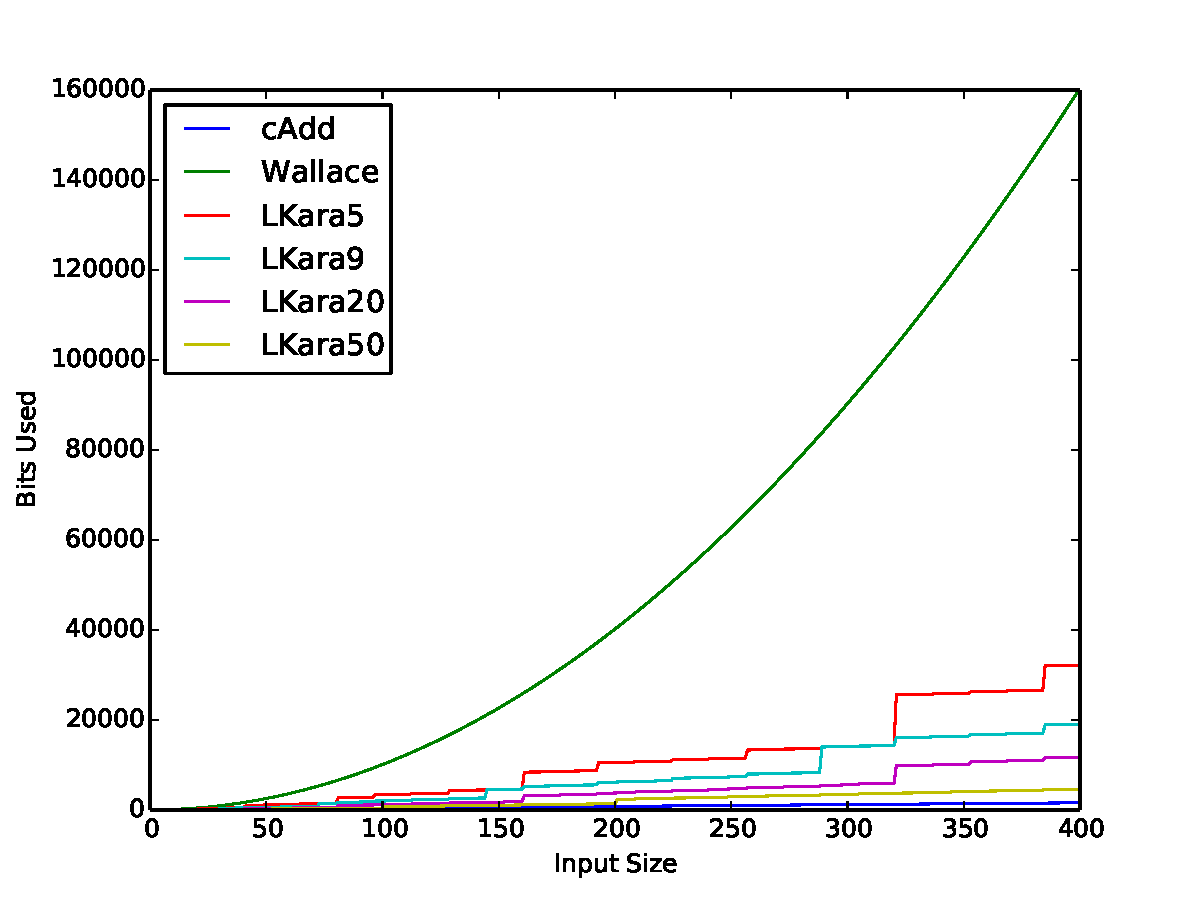
\includegraphics[width=\textwidth]{images/LKaraSize} 
        \caption{Plot of bits used verses input size for various Karatsuba cutoffs}
        \label{fig:size}
      \end{subfigure}
      \hfill
      \begin{subfigure}[b]{0.45\textwidth}
        \capstart
        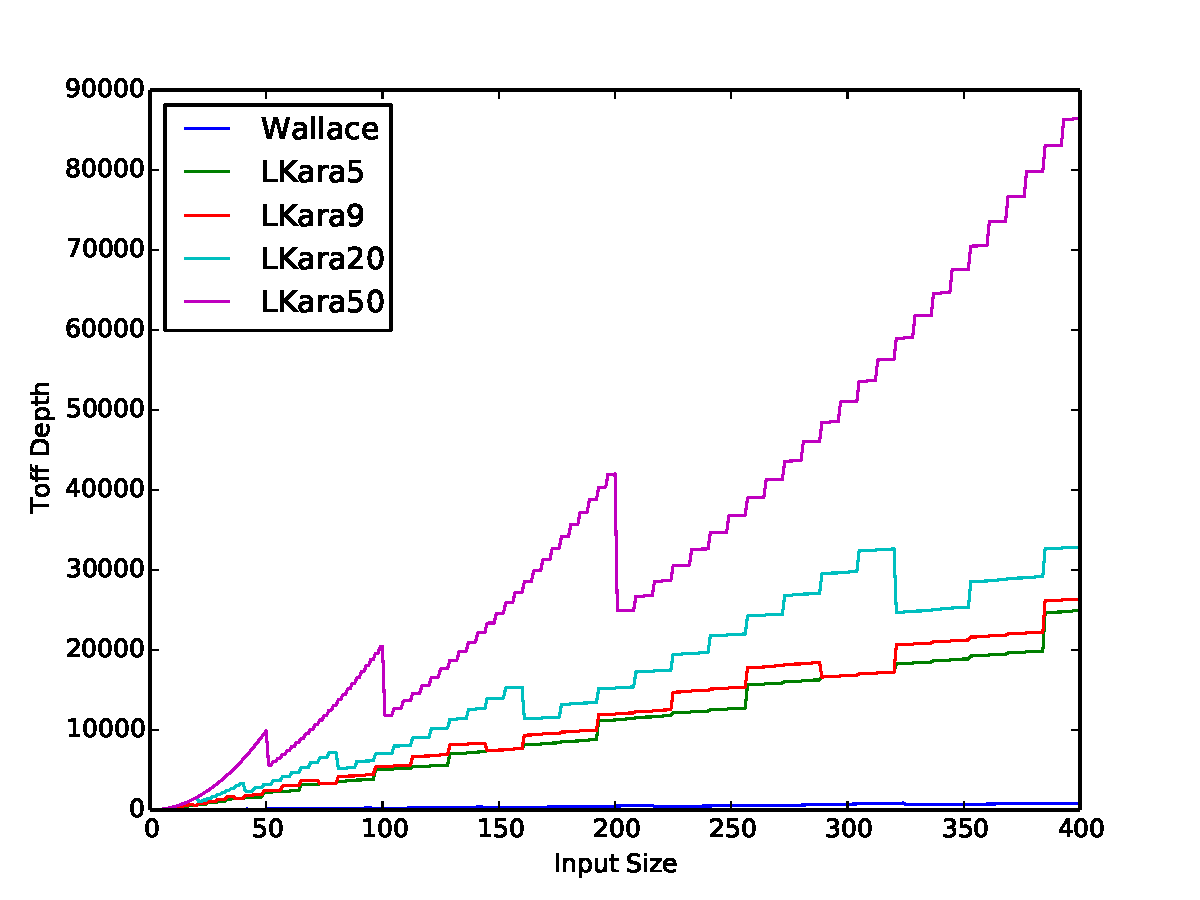
\includegraphics[width=\textwidth]{images/LKaraDepth2} 
        \caption{Plot of Toffoli depth verses input size for various Karatsuba cutoffs}
        \label{fig:depth}
      \end{subfigure}
      \caption{}
      \end{figure}

    \subsubsection{Depth}
      The Wallace tree achieves the best asymptotic depth.

\section{Division}
  \subsection{Simple binary integer division}
    In figure XXX is a simple integer division circuit based on the binary form of long division as outlined in algorithm \ref{algo:intdiv}.
    \begin{program}
      \capstart
      \caption{Integer Division with Remainder: find $R$ and $Q$ for $N/D$}
      \begin{algorithmic}[1]
        \Require $D \neq 0$
        \State $Q \gets 0$              
        \State $R \gets 0$                 
        \For{$i = n-1 \dots 0$}
          \State $R \gets R \ll 1$  
          \State $R(0) \gets N(i)$ \label{line:intdiv:setToN} 
          \If{$R \geq D$} \label{line:intdiv:compare}
            \State $R\gets R - D$               
            \State $Q(i) \gets 1$ \label{line:intdiv:setQ}

          \EndIf
        \EndFor 
      \end{algorithmic}
      \label{algo:intdiv}
    \end{program}
    An interesting feature of this algorithm is that combined with an in-place adder\cite{CDKM:2004} it can easily be made partially in-place.

    On \cref{line:intdiv:setToN} instead of allocating new space for $R(0)$ we can just use $N(i)$ as $R(0)$ since it will not be used again in the algorithm. 
    In doing this we will overwrite the value of $N$ with $R$ as the algorithm is run.
    The if statement on \Cref{line:intdiv:compare} can be preformed with a comparison circuit.  
    The result bit can be used to control the subtraction $R-D$.
    The value of the result bit is the same as $Q(i)$ after the assignment on \ref{line:intdiv:setQ}, so $Q(i)$ can just be taken to be the result bit. 
    This avoids additional ancilla and the assignment to $Q(i)$.


\section{Trigonometric functions}
    \subsection{CORDIC} 
        The basic idea of the CORDIC\cite{V:1959} algorithm is to apply repeated rotations which converge on a desired value.
        \[ \theta = \alpha_0 + \alpha_1 + \dotsb + \alpha_{n-1} \]
        The issue is that computing rotations is generally expensive;
        requiring multiplications and the evaluation of trig functions (the very thing we are using it to accomplish!).
        These rotation angles will be chosen such that this problem is avoided.

        A rotation matrix is given by:
        \[
          R_i = \begin{bmatrix}
            \cos\gamma_i & -\sin\gamma_i \\
            \sin\gamma_i & \cos\gamma_i
          \end{bmatrix}
        \]
        Using trig identities we can simplify this to 
        \[
          R_i = K_i
                \begin{bmatrix}
                  1            & -\tan\gamma_i \\
                  \tan\gamma_i & 1 
                \end{bmatrix}
        \]
        Where $K_i = \frac{1}{\sqrt{1+\tan^2\gamma_i}}$.

        We can collect all the $K_i$ terms into a single pre-computed scaling factor:
        \[ K(n) = \prod_{i=0}^{n-1}K_i \] 
        This can be applied with a single multiplication after the computation is complete.

        We can select $\gamma_i = \tan^{-1}2^{-i}$ as our set of angles so that all multiplications can be done simply as bit shifts. 
        These angles will be pre-computed 
        All that is left to do is find the directions of rotation.
        We can approximate some angle $\theta$ with the iterative process: $\theta_{i+1} = \theta_i + \sigma_i\gamma_i$.
        We choose the rotation direction $\sigma$ by comparing $\theta_i$ with $\theta$.
        If $\theta_i$ is greater then $\theta$ we rotate in the negative direction.
        If $\theta_i$ is less then then $\theta$ we rotate in the positive direction.

        This iterative process can be stated as:
        \begin{equation}\label{eq:cordIter}
            \begin{aligned}        
                x_{i+1}      &= x_i - \sigma_iy_i2^{-i}\\
                y_{i+1}      &= y_i + \sigma_ix_i2^{-i}\\
                \theta_{i+1} &= \theta_i - \sigma_i\gamma_i
            \end{aligned}
        \end{equation}

    \subsubsection{Reversible Implementation}
        The CORDIC algorithm can be implemented reversibly.

        We pre-compute all of our rotation angles ($\gamma_0,\gamma_1,\dotsc,\gamma_{n-1}$) as well as the scaling factor $K(n)$.

        Our input is the angle $\theta$ and our output is ($x$,$y$) where $\tan\theta = y/x$.

        \paragraph{Finding the directions of rotation}
            The directions of rotation can be determined using the sign bit of $\theta$.  
            At each step we copy out the sign bit of $\theta$ then add the angle $\gamma_i$ if $\theta$ is negative or subtract if it is positive.
            At the end the copied out set of bits $\sigma$ determine the directions of rotation.
            $\theta$ will approach zero so the higher order bits could possibly be cleaned up at the end of the step.
            Figure \ref{fig:CORDICDirections} shows a circuit for calculating $\sigma$.
            \begin{figure}[ht]
                \capstart
                \centering
                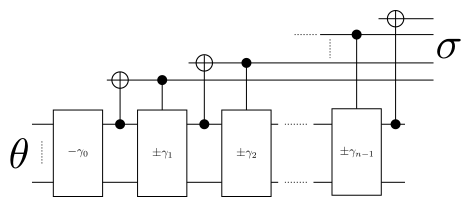
\includegraphics[width=\textwidth]{images/CORDICDirections} 
                \caption{Circuit to determine directions of rotation.  The controls determine whether $\gamma$ is added or subtracted.}
                \label{fig:CORDICDirections}
            \end{figure}

        \paragraph{Preforming Rotations}
            The actual rotation section is done using the iterative process above (\ref{eq:cordIter}).

            This circuit is shown in figure \ref{fig:CORDICRotations}.
            \begin{figure}[ht]
                \capstart
                \centering
                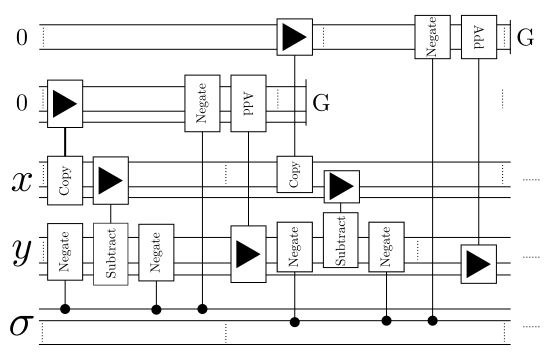
\includegraphics[width=\textwidth]{images/CORDICRotations} 
                \caption{Circuit to determine preform Rotations. 
                         $x$ and $y$ are both intialized to $1/\sqrt{2}$.
                         Garbage is cleaned at the end by copying out the result and repeating the circuit.}
                \label{fig:CORDICRotations}
            \end{figure}
        \subsubsection{Analysis}

\section{Converting OR to XOR}\todo{Reference revs paper}
In the case of mutually exclusive statements XOR is equivalent to OR.
That is to say $a \lor b = a \oplus b$ if $a = 1 \implies b = 0$ and $b = 1 \implies a =0$.  
For example $a\land b \lor \neg a \land c = a\land b \oplus \neg a \land c$. 

This is very useful as it allows us to avoid the use of Toffoli gates and use less ancilla.
For example if we wished to compute $a \lor b \lor c$ we might use the circuit:

  \[
    \Qcircuit @C=1em @R=.7em {
        \lstick{a} & \ctrlo{3} & \qw      & \ctrlo{3} & \rstick{a}\qw\\
        \lstick{b} & \ctrlo{2} & \qw      & \ctrlo{2} & \rstick{b}\qw\\
        \lstick{c} & \qw       & \ctrlo{2}& \qw       & \rstick{c}\qw\\
        \lstick{0} & \targ     & \ctrl{1} & \targ     & \rstick{0}\qw \\
        \lstick{0} & \qw       & \targ    & \targ      & \rstick{a \lor b \lor c}\qw
    }
  \]

Where as $a \oplus b \oplus c$ can be computed as:

\[
    \Qcircuit @C=1em @R=.7em {
        \lstick{a} & \ctrl{3}  & \qw      & \qw      & \rstick{a}\qw\\
        \lstick{b} & \qw       & \ctrl{2} & \qw      & \rstick{b}\qw\\
        \lstick{c} & \qw       & \qw      & \ctrl{1} & \rstick{c}\qw\\
        \lstick{0} & \targ     & \targ    & \targ    & \rstick{a \oplus b \oplus c}\qw \\
    }
\]

Or if one of $a$, $b$, or $c$. Are not needed in the later computation it can be done in-place as:

 \[
    \Qcircuit @C=1em @R=.7em {
        \lstick{a} & \ctrl{2}  & \qw      & \rstick{a}\qw\\
        \lstick{b} & \qw       & \ctrl{1} & \rstick{b}\qw\\
        \lstick{c} & \targ     & \targ    & \rstick{a \oplus b \oplus c}\qw \\
    }
\]

Given a set of AND expressions that are combined using OR we want to find sets of mutually exclusive statements that minimize the use of AND.
We consider each AND expression to be a vertex on a graph and add edges between vertices that are mutually exclusive.
Now we cover this graph using a minimum number of cliques.

After finding these cliques each set of mutually exclusive statements can be implemented by evaluating the AND statements and combining all of the values on a single ancilla using XOR for each clique.
These results can then be combined using OR statements (since OR is associative it does not matter how we group the statements). 

This algorithm has been implemented and tested on the BLIF benchmarks. \todo{add reference}
The results are shown below:
\todo{chart}

\section{Find First\label{sec:findFirst}} 
  Suppose you want to preform a set of functions which return some boolean value and you wish to know the first such function which returns $0$.
  For example if we have an $n$-bit number and we wish to find the position of the first $0$ value.

  In this case we want a controlled increment function that stop incrementing the first time the control is $0$.
  We therefore want to change the state of the counter by looking at just enough information to verify that all previous steps have been preformed.
  To do this we must look at a subset whose value is unique to the previous step.
  Note some difficulty is introduced by the reversible nature of the circuit in that we cannot depend on parts of the state that we are updating.
  To do this we simply follow a binary counting method which flips one bit each step (Grey Code).
  Since only one bit is flipped per iteration the context of the unflipped bits is sufficient to verify the previous steps. 
  An example of such a chain is shown below where the underlined portions of the state are the ones verified before the next step: 
  \[ 
    000 \to 00\underline{1} \to 0\underline{1}1 \to 0\underline{10} \to \underline{1}10 \to 
    \underline{1}1\underline{1} \to \underline{10}1 \to 100
  \]
